\chapter{New Material on Hopfield}
\chapterauthor{Scott Hotton, Jeff Yoshimi}

\section{New Material on Hopfield Networks}

   For a discrete Hopfield network we denote the input of neuron $n$ by $x_n$ 
and the output by $y_n$.  Neuron states are updated using an input-output 
relation.  If the input to neuron $n$ is below the threshold $U_n$ then the
output from neuron $N$ is $0$, otherwise the output is $1$.  This input-output
relation can be concisely expressed as:
\begin{equation}\label{E:hopIO}
   y_n(t+1) = 
\left\{
\begin{array}{ll}
0 & \mbox{if} \quad x_n(t) \leq U_n   \\
1 & \mathrm{otherwise} 
\end{array}\right.
\end{equation}
The threshold $U_n$ is often set to $0$ for all of the nodes.  So $y_n(t+1)$ is 
$0$ if $x(t)$ is not positive and it $1$ if $x(t)$ is positive.  

   The output of each neuron is an input for every neuron aside from itself.
The inputs are a linear combination of the state vector $(y_1, y_2, \ldots,
y_N)^T$ plus an input vector from the external environment.  The contribution
from each neuron is given by the weight matrix for the network.  The weight
matrix is is obtained as follows.

   Some of the vertices of an $N$ dimensional hypercube are chosen to be the 
attracting fixed points for a network.  The vertex for the $n^{\mathrm{th}}$ 
object is denoted by 
\begin{equation*}
\boldsymbol{p}_n =
\begin{pmatrix}
p_{1n} \\ p_{2n} \\ \vdots \\ p_{Nn}
\end{pmatrix}
\end{equation*}
for $n = 1,2, \ldots, N$.  In order for $\boldsymbol{p}_n$ to be a vertex
of the hypercube $[0,1]^N$ we need $p_{jn}$ to be $0$ or $1$ for all $j$, $n 
\in \{1, \ldots, N\}$.

   In a Hopfield network the weight of a neuron to itself is always $0$.
Otherwise the general formula the weights is:
\begin{equation}\label{E:hopweights}
w_{jk} = \sum_{n=1}^N (2 p_{nj} - 1)(2 p_{nk} - 1) 
\end{equation}
for all $j$, $k \in \{1, \ldots, N\}$ and $j \neq k$.  It follows that 
$w_{jk} = w_{kj}$ for all $j$, $k \in \{1, \ldots, N\}$ and that the weight 
matrix for a Hopfield network is symmetric.  

   The input to each neuron is a weighted combination of the activations for 
all of the other neurons plus a term for the external environment which we 
assume here is constant.  We let $I_n$ denote the external input and 
$(I_1, I_2, \ldots, I_n)^T$ denote the vector of fixed inputs to the $N$ nodes 
in the neural network.  The inputs to the neurons at time $t$ can be expressed
concisely as:
\begin{equation}\label{E:hopinput}
\begin{pmatrix}
x_1(t) \\  x_2(t) \\ \vdots \\ x_N(t)
\end{pmatrix}
 = 
 \begin{pmatrix} 
     0      & w_{12} & \cdots & w_{1N} \\ 
     w_{12} &   0    & \cdots & w_{2N} \\ 
     \vdots & \vdots & \ddots & \vdots \\ 
     w_{1N} & w_{2N} & \cdots &   0  
 \end{pmatrix} 
 \begin{pmatrix} 
     y_1(t) \\ y_2(t) \\ \vdots \\ y_N(t) 
  \end{pmatrix} 
     +
\begin{pmatrix}
I_1 \\  I_2 \\ \vdots \\ I_N
\end{pmatrix}
\end{equation}
A Hopfield network operates by successively applying rules \eqref{E:hopinput} 
and \eqref{E:hopIO}.

\subsection{Types of Update}

   The rules \eqref{E:hopinput} and \eqref{E:hopIO} can be apply synchronously
or asynchronously.  With synchronous update rules \eqref{E:hopinput} and 
\eqref{E:hopIO} are successively applied to all of the neurons at the same 
time.  For a fixed input vector this gives us a function from the state space 
to itself.  By iterating this function we obtain a dynamical system on the 
neural network's state space.  With synchronous update the states chosen to be
the attracting fixed points do become attracting fixed points for the 
appropriate inputs.

   Synchronous update is not used very often because it allows the neural
network to become stuck in oscillations when more than one object is present 
in the environment.  So it can not decide whether an object is present or not.
Instead of updating all of the neurons in a Hopfield network at the same time 
we can update them one at a time.  Hopfield proposed two ways to do this.  One 
way is to go through each of neurons in the network in some fixed order.  This 
is called \emph{sequential update}.  We choose a sequence for the neurons in 
the network.  The chosen sequence is usually finite in length and when we reach 
the end of the sequence we start again at the beginning.  We update the neurons 
by repeatedly going through the chosen sequence.  The other way is to select 
neurons in the network randomly.  This is called \emph{stochastic update}.

   For a fixed input vector and chosen neuron the update rules specify a 
function from the state space to itself.  With sequential update we get a 
sequence of functions from the state space to itself as we go through the 
chosen sequence for the neurons.  Composing the sequence of functions we get 
for updating each individual neuron gives us a function from the state space to 
itself.  We can iterate this function to obtain a dynamical system on the 
neural network's state space.

   In general we do not get a single dynamical system from sequential update.
The dynamical systems that we generally get depend on the sequence we choose
for updating the neurons.  This means that the dynamical systems we generally
get with sequential update are different from the dynamical system we get with
synchronous update.  The dynamical systems obtained using sequential update 
tend to only have fixed point attractors.  They do not get stuck oscillating 
between two or more states.

   Stochastic update uses a chosen probability distribution on the set of 
neurons.  The neurons are randomly selected one at a time so that their 
frequency of occurrence follows the chosen probability distribution.  The
chosen probability distribution is usually the uniform distribution on the 
set of neurons.  In this case each neuron has the same chance of being selected
for update. 

   For a fixed input vector, $(I_1, I_2, \ldots, I_N)^T$, and randomly selected
neuron $n$, the update rules specify a function from the state space to itself.
However stochastic update does not give us a dynamical system on the state 
space of the neural network.  Rather it gives us a Markov process on the state 
space.  A Markov process is a stochastic process in which the probability for
next state in time only depends on the present state.  The probability of 
going from one state to another is called a transition probability.  There is
a transition probability for every pair of states.  The transition 
probabilities can sometimes be $0$ or $1$.

   So long as the inputs are fixed the future state of a discrete Hopfield 
network only depends on which neuron was selected.  With stochastic update 
the neurons are selected randomly so we get a stochastic process in which the
probability for the next state only depends in the present state.  So 
stochastic update gives us a Markov process.  Its actually a fairly simple
type of Markov process in which there are states where the transition
probability to themselves is $1$.  These are called absorbing states.  Once a
Markov process enters an absorbing state it will almost certainly stay there
for all future times.  A discrete Hopfield network with stochastic update will 
almost certainly end up in an absorbing state as time increases without bound.
In this sense the network is able to decide whether an object is present or 
not, despite having some randomness.

\subsection{Hopfield's Potential Function}

  Hopfield's potential function for an arbitrary discrete Hopfield network 
can be concisely expressed as:
\begin{equation}
V
\begin{pmatrix}
y_1 \\  y_2 \\ \vdots \\ y_N
\end{pmatrix}
  =  -\,\displaystyle{\frac{1}{2}} \left(
     \begin{matrix}
       \begin{pmatrix}
           y_1 & y_2 & & \cdots & y_N 
       \end{pmatrix} \\ \\ \\ \mbox{}\end{matrix}
       \begin{pmatrix} 
           0      & w_{12} & \cdots & w_{1N} \\ 
           w_{12} &   0    & \cdots & w_{2N} \\ 
           \vdots & \vdots & \ddots & \vdots \\ 
           w_{1N} & w_{2N} & \cdots &   0  
       \end{pmatrix} 
       \begin{pmatrix} 
            y_1 \\ y_2 \\ \vdots \\ y_N 
       \end{pmatrix} 
     \right) -
\begin{pmatrix}
I_1 \\  I_2 \\ \vdots \\ I_N
\end{pmatrix}
\bullet
\begin{pmatrix}
y_1 \\  y_2 \\ \vdots \\ y_N
\end{pmatrix}
\end{equation}
This quantity never increases and states chosen to be the attracting fixed 
points are local minima for the appropriate inputs.
  
\subsection{A discrete Hopfield network with two neurons}

   In this section we present a simple example of a discrete Hopfield network
with two neurons.  Many of the properties of Hopfield networks can be observed
in a network with just two neurons.  We will train the Hopfield network to 
detect the presence or absence of two objects.  As with the example Hopfield 
network with continuous neurons we choose the attracting fixed points to be a 
pair of opposite vertices in the square $[0,1]^2$.  
\begin{equation*}
\boldsymbol{p}_1 = 
\begin{pmatrix}
p_{11} \\ p_{12}
\end{pmatrix}
=
\begin{pmatrix}
1 \\ 0
\end{pmatrix}
\qquad \mathrm{and} \qquad
\boldsymbol{p}_2 = 
\begin{pmatrix}
p_{21} \\ p_{22}
\end{pmatrix}
=
\begin{pmatrix}
0 \\ 1
\end{pmatrix}
\end{equation*}
Only the connections between the two neurons can have nonzero weights and by 
symmetry those connections have the same weight.  By formula 
\eqref{E:hopweights} the nonzero weight is:
\begin{equation*}
w_{12} = w_{21} = 
 (2 \cdot 1 - 1)(2  \cdot 0 - 1) + (2 \cdot 0 - 1)(2 \cdot 1  - 1)
 = (1)(-1) + (-1)(1) = -2
\end{equation*}
So the weight matrix for this Hopfield network is:
\begin{equation*}
\begin{pmatrix}
 0 & -2 \\
-2 &  0 
\end{pmatrix}
\end{equation*}
The formula for the neuron inputs in terms of their states can be simplified 
to:
\begin{equation*}
\begin{pmatrix}
x_1(t) \\ x_2(t)
\end{pmatrix}
=
\begin{pmatrix}
 0 & -2 \\
-2 &  0 
\end{pmatrix}
\begin{pmatrix}
y_1(t) \\ y_2(t)
\end{pmatrix}
+
\begin{pmatrix}
I_1 \\ I_2
\end{pmatrix}
=
\begin{pmatrix}
I_1 - 2 y_2(t) \\ I_2 - 2 y_1(t)
\end{pmatrix}
\end{equation*}

%   We chose $U_1=U_2=0$ in equation \eqref{E:hopIO}.  The 
%inequality $I_1 - 2 y_2(t) \leq 0$ is algebraically equivalent to the 
%inequality $y_2(t) \geq I_1/2$ and the inequality $I_2 - 2 y_1(t) \leq 0$ is 
%algebraically equivalent to the inequality $y_1(t) \geq I_2/2$.  We can use 
%these latter inequalities to express the result of applying rules 
%\eqref{E:hopinput} and \eqref{E:hopIO}.  This is a function that gives us the 
%state $(y_(t+1),y_2(t+1))^T$ from the state $(y_(t),y_2(t))^T$.  
%
%   By rule \eqref{E:hopinput} the quantity $x_1(t) = I_1 - 2 y_2(t)$.  So for
%instance, if $y_2(t)\geq I_1/2$ then $x_1(t) \leq 0$ and therefore $y_1(t+1) = 
%0$ by rule \eqref{E:hopIO}.  By the same reasoning if $y_1(t)\geq I_2/2$ then 
%$y_2(t+1) = 0$.  So if $y_1(t)\geq I_2/2$ and $y_2(t)\geq I_1/2$ then 
%$(y_1(t+1),y_2(t+1))^T = (0,0)^T$.  We leave it as an exercise to show that
%the function for $(y_1(t+1), y_2(t+1))^T$ in terms of $(y_(t),y_2(t))^T$ is:
%\begin{equation}\label{E:hopexam}
%\begin{pmatrix}
%y_1(t+1) \\ y_2(t+1)
%\end{pmatrix}
%= 
%F
%\left(
%\begin{pmatrix}
%y_1(t) \\ y_2(t)
%\end{pmatrix},
%\begin{pmatrix}
%I_1 \\ I_2
%\end{pmatrix}
%\right)
%=
%\left\{
%\begin{array}{ll}
%(0,0)^T & \mbox{if} \quad y_1(t) \geq I_2/2 \quad 
%          \mbox{and} \quad y_2(t) \geq I_1/2 \\
%(1,0)^T & \mbox{if} \quad y_1(t) \geq I_2/2 \quad 
%          \mbox{and} \quad y_2(t) < I_1/2 \\
%(0,1)^T & \mbox{if} \quad y_1(t) < I_2/2 \quad 
%          \mbox{and} \quad y_2(t) \geq I_1/2 \\
%(1,1)^T & \mbox{if} \quad y_1(t) < I_2/2 \quad 
%          \mbox{and} \quad y_2(t) < I_1/2
%\end{array}\right.
%\end{equation}
%for any fixed input $(I_1,I_2)^T \in \bf{R}^2$.  Iterating the function $F$ 
%gives us a parameterized family of dynamical systems for the Hopfield network 
%with the fixed inputs as the parameters.
%
   With just two neurons we can compute the response of this neural network to 
a given input by using equation \eqref{E:hopexam}.  For each of the update 
methods, synchronous, sequential, and stochastic we will consider four input 
vectors:
\begin{equation*}
\begin{pmatrix}
I_1 \\ I_2
\end{pmatrix}
= 
\begin{pmatrix}
0 \\ 0
\end{pmatrix}, \qquad 
\begin{pmatrix}
I_1 \\ I_2
\end{pmatrix}
= 
\begin{pmatrix}
1 \\ 0
\end{pmatrix}, \qquad 
\begin{pmatrix}
I_1 \\ I_2
\end{pmatrix}
= 
\begin{pmatrix}
0 \\ 1
\end{pmatrix}, \qquad 
\mbox{and}  \qquad 
\begin{pmatrix}
I_1 \\ I_2
\end{pmatrix}
= 
\begin{pmatrix}
1 \\ 1
\end{pmatrix}
\end{equation*}

\subsubsection{Synchronous update} 

%\bigskip
%\noindent
%{\bf Case} $(I_1,I_2)^T = (0,0)^T$.  
%\bigskip
%
%   Equation \eqref{E:hopexam} becomes 
%\begin{equation*}
%\begin{pmatrix}
%y_1(t+1) \\ y_2(t+1)
%\end{pmatrix}
%= 
%F
%\left(
%\begin{pmatrix}
%y_1(t) \\ y_2(t)
%\end{pmatrix},
%\begin{pmatrix}
%0 \\ 0
%\end{pmatrix}
%\right)
%=
%\left\{
%\begin{array}{ll}
%(0,0)^T & \mbox{if} \quad y_1(t) \geq 0 \quad \mbox{and} \quad y_2(t) \geq 0 \\
%(1,0)^T & \mbox{if} \quad y_1(t) \geq 0 \quad \mbox{and} \quad y_2(t) < 0    \\
%(0,1)^T & \mbox{if} \quad y_1(t) < 0 \quad \mbox{and} \quad y_2(t) \geq 0 \\
%(1,1)^T & \mbox{if} \quad y_1(t) < 0 \quad \mbox{and} \quad y_2(t) <  0 
%\end{array}\right.
%\end{equation*}
%The inequalities 
%\begin{equation*}
%y_1(t) \geq 0 \quad \mbox{and} \quad y_2(t) \geq 0 
%\end{equation*}
%hold for all $(y_1(t),y_2(t))^T \in \{0,1\}^2$ so all states go to $(0,0)^T$ 
%in a single time step.  When the input vector is $(0,0)^T$ the neural network 
%goes to the state $(0,0)^T$ as we wanted.
%
%\bigskip
%\noindent
%{\bf Case} $(I_1,I_2)^T = (1,0)^T$.  
%\bigskip
%
%   Equation \eqref{E:hopexam} becomes 
%\begin{equation*}
%\begin{pmatrix}
%y_1(t+1) \\ y_2(t+1)
%\end{pmatrix}
%= 
%F
%\left(
%\begin{pmatrix}
%y_1(t) \\ y_2(t)
%\end{pmatrix},
%\begin{pmatrix}
%1 \\ 0
%\end{pmatrix}
%\right)
%=
%\left\{
%\begin{array}{ll}
%(0,0)^T & \mbox{if} \quad y_1(t) \geq 0 \quad \mbox{and} \quad y_2(t) \geq 1/2 \\
%(1,0)^T & \mbox{if} \quad y_1(t) \geq 0 \quad \mbox{and} \quad y_2(t) < 1/2 \\
%(0,1)^T & \mbox{if} \quad y_1(t) < 0 \quad \mbox{and} \quad y_2(t) \geq 1/2 \\
%(1,1)^T & \mbox{if} \quad y_1(t) < 0 \quad \mbox{and} \quad y_2(t) < 1/2 
%\end{array}\right.
%\end{equation*}
%\indent Computing this gives:
%\begin{eqnarray*}
%&F
%\left(
%\begin{pmatrix}
%0 \\ 1 
%\end{pmatrix},
%\begin{pmatrix}
%1 \\ 0 
%\end{pmatrix}
%\right)
%=
%\begin{pmatrix}
%0 \\ 0 
%\end{pmatrix}, \qquad
% F
%\left(
%\begin{pmatrix}
%1 \\ 1 
%\end{pmatrix},
%\begin{pmatrix}
%1 \\ 0 
%\end{pmatrix}
%\right)
%=
%\begin{pmatrix}
%0 \\ 0 
%\end{pmatrix} & \\
%& 
%F
%\left(
%\begin{pmatrix}
%0 \\ 0 
%\end{pmatrix},
%\begin{pmatrix}
%1 \\ 0 
%\end{pmatrix}
%\right)
%=
%\begin{pmatrix}
%1 \\ 0 
%\end{pmatrix}, \qquad
%F
%\left(
%\begin{pmatrix}
%1 \\ 0 
%\end{pmatrix},
%\begin{pmatrix}
%1 \\ 0 
%\end{pmatrix}
%\right)
%=
%\begin{pmatrix}
%1 \\ 0 
%\end{pmatrix}& 
%\end{eqnarray*}
%\indent The state $(1,0)$ is a globally attracting fixed point as we wanted 
%for the input $(1,0)^T$.
%
%\bigskip
%\noindent
%{\bf Case} $(I_1,I_2)^T = (0,1)^T$.  
%\bigskip
%
%   Equation \eqref{E:hopexam} becomes 
%\begin{equation*}
%\begin{pmatrix}
%y_1(t+1) \\ y_2(t+1)
%\end{pmatrix}
%= 
%F
%\left(
%\begin{pmatrix}
%y_1(t) \\ y_2(t)
%\end{pmatrix},
%\begin{pmatrix}
%0 \\ 1
%\end{pmatrix}
%\right)
%=
%\left\{
%\begin{array}{ll}
%(0,0)^T & \mbox{if} \quad y_1(t) \geq 1/2 \quad \mbox{and} \quad y_2(t) \geq 0 \\
%(1,0)^T & \mbox{if} \quad y_1(t) \geq 1/2 \quad \mbox{and} \quad y_2(t) < 0 \\
%(0,1)^T & \mbox{if} \quad y_1(t) < 1/2 \quad \mbox{and} \quad y_2(t) \geq 0 \\
%(1,1)^T & \mbox{if} \quad y_1(t) < 1/2 \quad \mbox{and} \quad y_2(t) < 0
%\end{array}\right.
%\end{equation*}
%\indent Computing this gives:
%\begin{eqnarray*}
%&F
%\left(
%\begin{pmatrix}
%0 \\ 1 
%\end{pmatrix},
%\begin{pmatrix}
%0 \\ 1 
%\end{pmatrix}
%\right)
%=
%\begin{pmatrix}
%0 \\ 1 
%\end{pmatrix}, \qquad
% F
%\left(
%\begin{pmatrix}
%1 \\ 1 
%\end{pmatrix},
%\begin{pmatrix}
%0 \\ 1 
%\end{pmatrix}
%\right)
%=
%\begin{pmatrix}
%0 \\ 0 
%\end{pmatrix} & \\
%& 
%F
%\left(
%\begin{pmatrix}
%0 \\ 0 
%\end{pmatrix},
%\begin{pmatrix}
%0 \\ 1 
%\end{pmatrix}
%\right)
%=
%\begin{pmatrix}
%0 \\ 1 
%\end{pmatrix}, \qquad
%F
%\left(
%\begin{pmatrix}
%1 \\ 0 
%\end{pmatrix},
%\begin{pmatrix}
%0 \\ 1 
%\end{pmatrix}
%\right)
%=
%\begin{pmatrix}
%0 \\ 0 
%\end{pmatrix}& 
%\end{eqnarray*}
%\indent The state $(0,1)$ is a globally attracting fixed point as we wanted for 
%the input $(0,1)$.
%
%\bigskip
%\noindent
%{\bf Case} $(I_1,I_2)^T = (1,1)^T$.  
%\bigskip
%
%   Equation \eqref{E:hopexam} becomes 
%\begin{equation*}
%\begin{pmatrix}
%y_1(t+1) \\ y_2(t+1)
%\end{pmatrix}
%= 
%F
%\left(
%\begin{pmatrix}
%y_1(t) \\ y_2(t)
%\end{pmatrix},
%\begin{pmatrix}
%1 \\ 1
%\end{pmatrix}
%\right)
%=
%\left\{
%\begin{array}{ll}
%(0,0)^T & \mbox{if} \quad y_1(t) \geq 1/2 \quad \mbox{and} \quad y_2(t) \geq 1/2 \\
%(1,0)^T & \mbox{if} \quad y_1(t) \geq 1/2 \quad \mbox{and} \quad y_2(t) < 1/2 \\
%(0,1)^T & \mbox{if} \quad y_1(t) < 1/2 \quad \mbox{and} \quad y_2(t) \geq 1/2 \\
%(1,1)^T & \mbox{if} \quad y_1(t) < 1/2 \quad \mbox{and} \quad y_2(t) < 1/2
%\end{array}\right.
%\end{equation*}
%\indent Computing this gives:
%\begin{eqnarray*}
%&F
%\left(
%\begin{pmatrix}
%0 \\ 1 
%\end{pmatrix},
%\begin{pmatrix}
%1 \\ 1 
%\end{pmatrix}
%\right)
%=
%\begin{pmatrix}
%0 \\ 1 
%\end{pmatrix}, \qquad
% F
%\left(
%\begin{pmatrix}
%1 \\ 1 
%\end{pmatrix},
%\begin{pmatrix}
%1 \\ 1 
%\end{pmatrix}
%\right)
%=
%\begin{pmatrix}
%0 \\ 0 
%\end{pmatrix} & \\
%& 
%F
%\left(
%\begin{pmatrix}
%0 \\ 0 
%\end{pmatrix},
%\begin{pmatrix}
%1 \\ 1 
%\end{pmatrix}
%\right)
%=
%\begin{pmatrix}
%1 \\ 1 
%\end{pmatrix}, \qquad
%F
%\left(
%\begin{pmatrix}
%1 \\ 0 
%\end{pmatrix},
%\begin{pmatrix}
%1 \\ 1 
%\end{pmatrix}
%\right)
%=
%\begin{pmatrix}
%1 \\ 0 
%\end{pmatrix}& 
%\end{eqnarray*}
%\indent There are two fixed points, $(1,0)^T$ and $(0,1)^T$, but the other two 
%states do not go to the fixed \\ 
%\indent points.  Instead the neural network's state goes back and forth between 
%the other two states.  \\
%\indent They form a $2$-cycle.
%
%\bigskip

   The dynamics on the state space of the neural network can be expressed with 
a digraph where the vertices are the four states of the neural network and each
vertex has exactly one directed edge pointing away from it.  This is shown in
Fig. \ref{F:TwoNodeHopfield}.  The directed edge pointing away from a vertex 
tells us what the subsequent state will be.

\begin{figure}[ht]
\centering
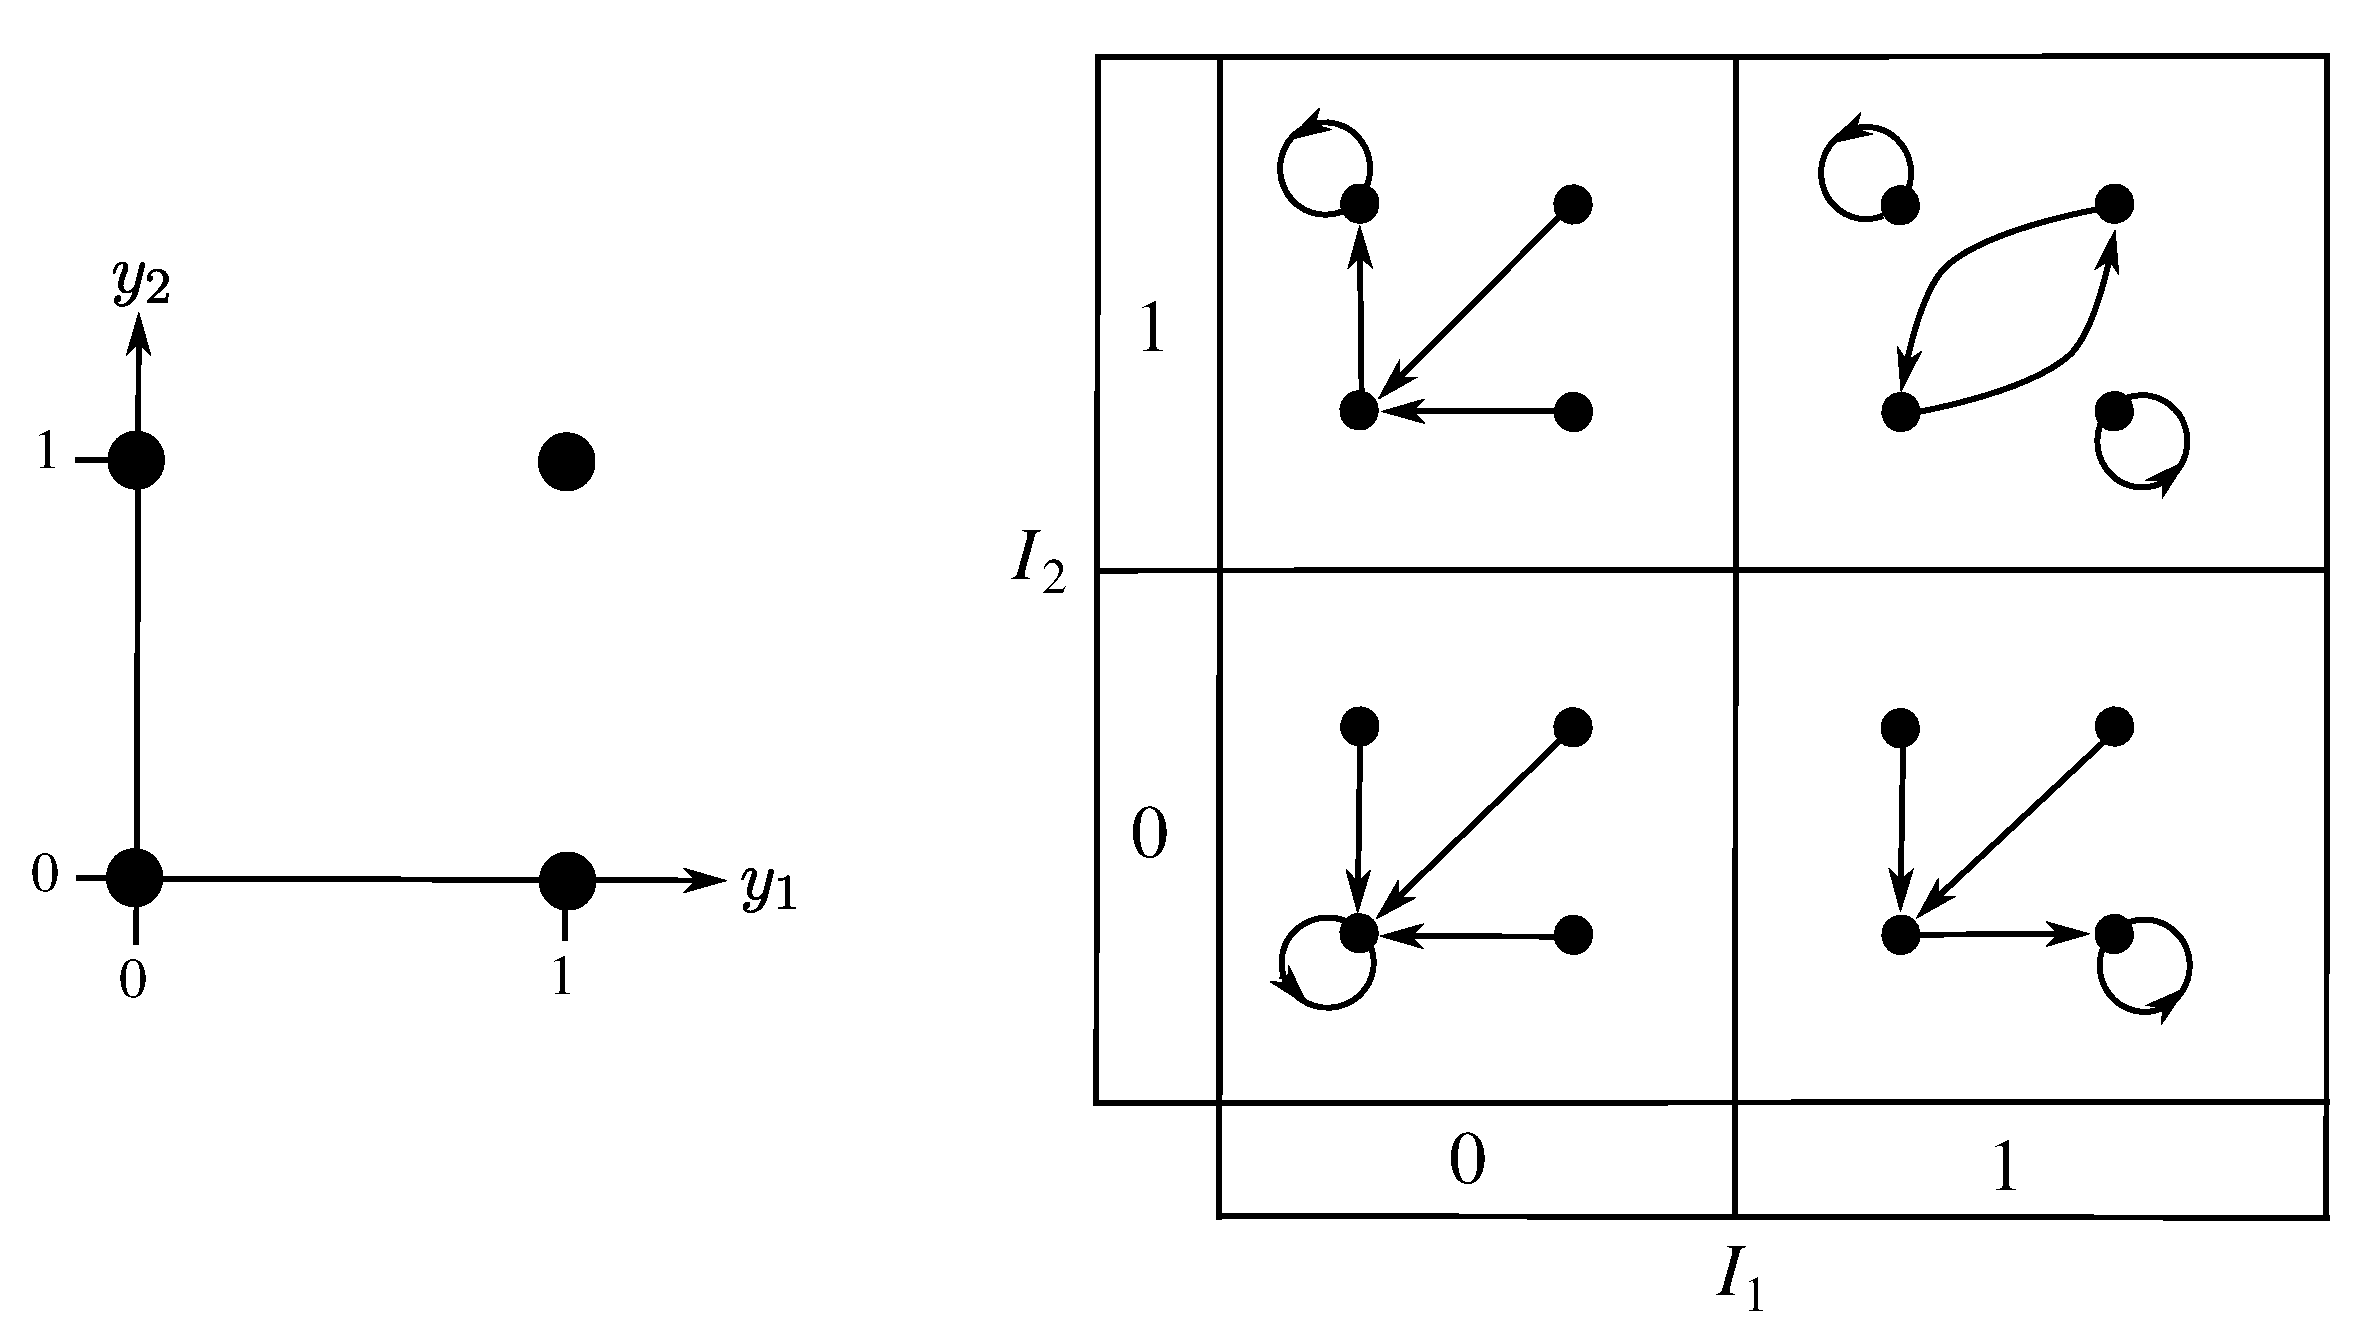
\includegraphics[scale=0.40]{./images/TwoNodeHopfield.pdf}
\caption{The dynamics for the Hopfield network with two discrete neurons. 
(Left) The state space for the neural network is the set of four vertices 
$\{0,1\}^2$.  (Right) The dynamics of the neural network is represented with 
digraphs on the state space for the four chosen input values for $(I_1,I_2)^T$. 
This is like a phase portrait for the discrete dynamical system.}
\label{F:TwoNodeHopfield}  
\end{figure}

   If both inputs are $0$ then the neural network goes to the state $(0,0)^T$ 
in one time step.  This state corresponds to the neural network recognizing 
that neither object is present.  If the input for the first object is $1$ and 
for the second object is $0$ then the neural network goes to the state $(1,0)$
in at most two time steps and once it is there it stays there, so long as the
inputs do not change.  This state corresponds to the neural network recognizing
that object 1 is present and object 2 is absent.  If the input for the first 
object is $0$ and for the second object is $1$ then the neural network goes to 
the state $(1,0)$ in at most two time steps and once it is there it 
stays there, so long as the inputs do not change.  This state corresponds to 
the neural network recognizing that object 2 is present and object 1 is absent.
In these three cases the neural network has a globally attracting fixed point
and it is the fixed point we want for the input.

   If both inputs are $1$ then the long term behavior depends on the state
that it is in during the present moment.  If it begins in a state that 
corresponds to recognizing the presence of one object and the absence of the 
other object then it will stay in that state for all time despite the fact that 
both objects are present\footnote{This resembles priming in perceptual 
psychology}.  If the network does not begin in a state that corresponds to 
recognizing the presence of one object and the absence of the other object then 
it will never go to such a state.  It will simply oscillate between the states 
$(0,0)^T$ and $(1,1)^T$\footnote{This resembles being in a confused mental 
state.}. 

   This neural network can recognize the absence of both objects and it can
recognize the presence of an object if the other object is absent.  If both
objects are present then it will only recognize an object if it is already in 
the state that corresponds to recognizing that object.  Otherwise it will
oscillate between the states $(0,0)^T$ and $(1,1)^2$.

  Hopfield's potential function is:
\begin{eqnarray*}
V
\begin{pmatrix}
y_1 \\  y_2
\end{pmatrix}
 &=& -\,\displaystyle{\frac{1}{2}} \left(
  \begin{matrix}\begin{pmatrix}y_1 & y_2\end{pmatrix}\\\mbox{}\end{matrix}
  \begin{pmatrix} 0 & -2 \\ -2 & 0 \end{pmatrix} 
  \begin{pmatrix} y_1 \\ y_2 \end{pmatrix} \right) 
-
\begin{pmatrix}
I_1 \\ I_2 
\end{pmatrix}
\bullet
\begin{pmatrix}
y_1 \\ y_2 
\end{pmatrix} \\
~ &=& 
  \begin{matrix}\begin{pmatrix}y_1 & y_2\end{pmatrix}\\\mbox{}\end{matrix}
  \begin{pmatrix} 0 & 1 \\ 1 & 0 \end{pmatrix} 
  \begin{pmatrix} y_1 \\ y_2 \end{pmatrix} 
-
\begin{pmatrix}
I_1 \\ I_2 
\end{pmatrix}
\bullet
\begin{pmatrix}
y_1 \\ y_2 
\end{pmatrix} = 2 y_1 y_2 - I_1 y_1 - I_2 y_2
\end{eqnarray*}
The values of the potential function on the state space $\{0,1\}^2$ can be
easily computed.  They are shown in Fig. \ref{F:discHoppot}.  The directed 
edges point to the subsequent state.  As can be seen from the figure the 
potential function never increases with time.  And each fixed point is a 
minimum of the potential although they are not always the only minima.

\begin{figure}[ht]
\centering
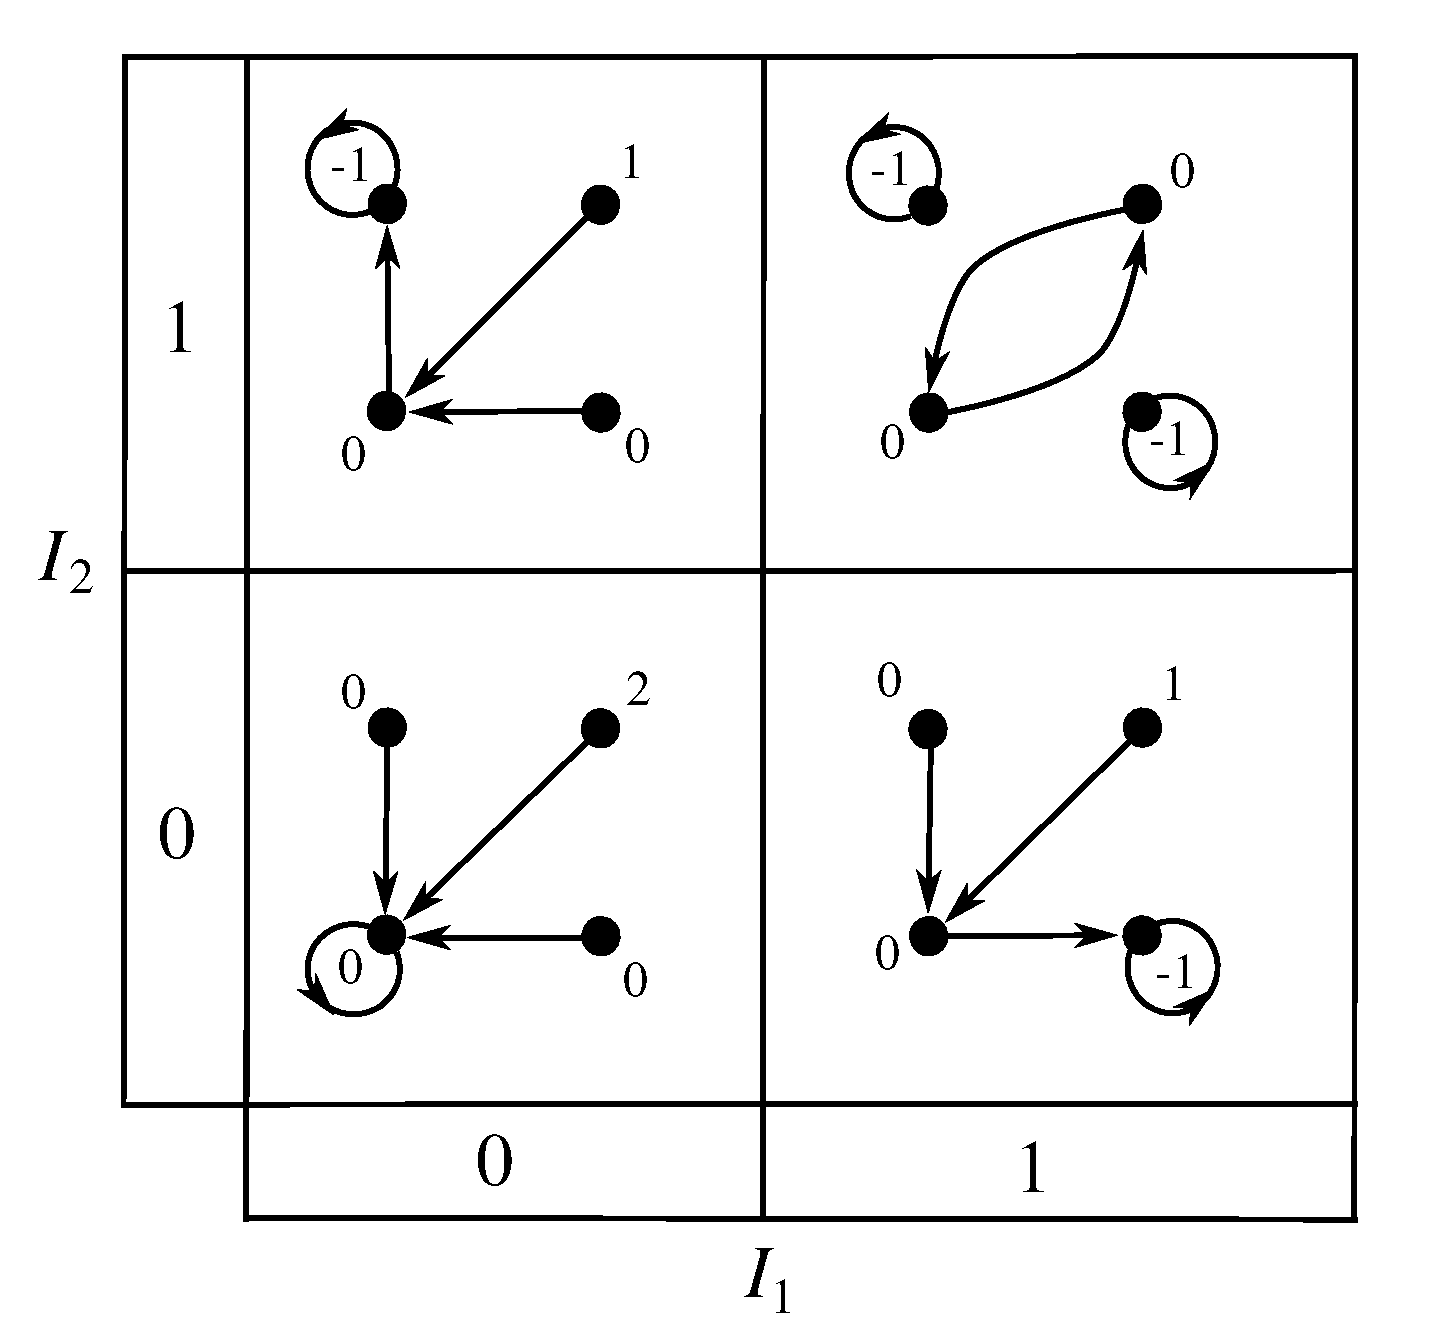
\includegraphics[scale=0.40]{./images/discHoppot.pdf}
\caption{The potential function $V(y_1, y_2)$ for the four chosen input 
values for $(I_1,I_2)^T$ along with the phase portrait.  The value of the 
potential function is labeled next to each state.}
\label{F:discHoppot}  
\end{figure}
  
\subsubsection{Asynchronous update}

   With asynchronous update we only update one neuron at a time in the neural 
network.  The two types of asynchronous update, sequential and stochastic,
only differ in how we select the neurons to update.  Let $n \in \{1,2\}$ stand 
for which neuron has been selected to be updated.  We still apply rules 
\eqref{E:hopinput} and \eqref{E:hopIO} to obtain a function that gives us the 
state $(y_1(t+1), y_2(t+1))^T$ in terms of the state $(y_1(t), y_2(t))^T$ but 
for rule \eqref{E:hopinput} we only use the component $x_n(t)$ in the vector 
$(x_1(t), x_2(t))^T$.  We then apply rule \eqref{E:hopIO} to $x_n(t)$ to get 
$y_n(t+1)$.

   The update function for neuron $1$ is:
\begin{equation}\label{E:hopexam1}
F_1
\left(
\begin{pmatrix}
y_1(t) \\ y_2(t)
\end{pmatrix},
\begin{pmatrix}
I_1 \\ I_2
\end{pmatrix}
\right)
=
\left\{
\begin{array}{ll}
(0,y_2(t))^T & \mbox{if} \quad y_2(t) \geq I_1/2 \\
(1,y_2(t))^T & \mbox{if} \quad y_2(t) < I_1/2 
\end{array}\right.
\end{equation}

   The update function for neuron $2$ is:
\begin{equation}\label{E:hopexam1}
F_2
\left(
\begin{pmatrix}
y_1(t) \\ y_2(t)
\end{pmatrix},
\begin{pmatrix}
I_1 \\ I_2
\end{pmatrix}
\right)
=
\left\{
\begin{array}{ll}
(y_1(t),0)^T & \mbox{if} \quad y_1(t) \geq I_2/2 \\
(y_1(t),1)^T & \mbox{if} \quad y_1(t) < I_2/2 
\end{array}\right.
\end{equation}
We can compute sequential update and stochastic update by composing these two 
functions on the state space $\{0,1\}^2$.  The digraphs for these two functions 
are shown in Fig.  \ref{F:TwoNodeHopfieldSingle}.  We can obtain the digraph 
for $F_1$ by using the formula for $F_1$ or by redirecting the arrows in Fig. 
\ref{F:discHoppot} so that only $y_1$ changes.  This is shown on the left in
Fig. \ref{F:TwoNodeHopfieldSingle}.  Similarly we can obtain the digraph for 
$F_2$ from the formula or by redirecting the arrows in Fig. \ref{F:discHoppot} 
so that only $y_2$ changes.  This is shown on the right in Fig.  
\ref{F:TwoNodeHopfieldSingle}.

\begin{figure}[ht]
\centering
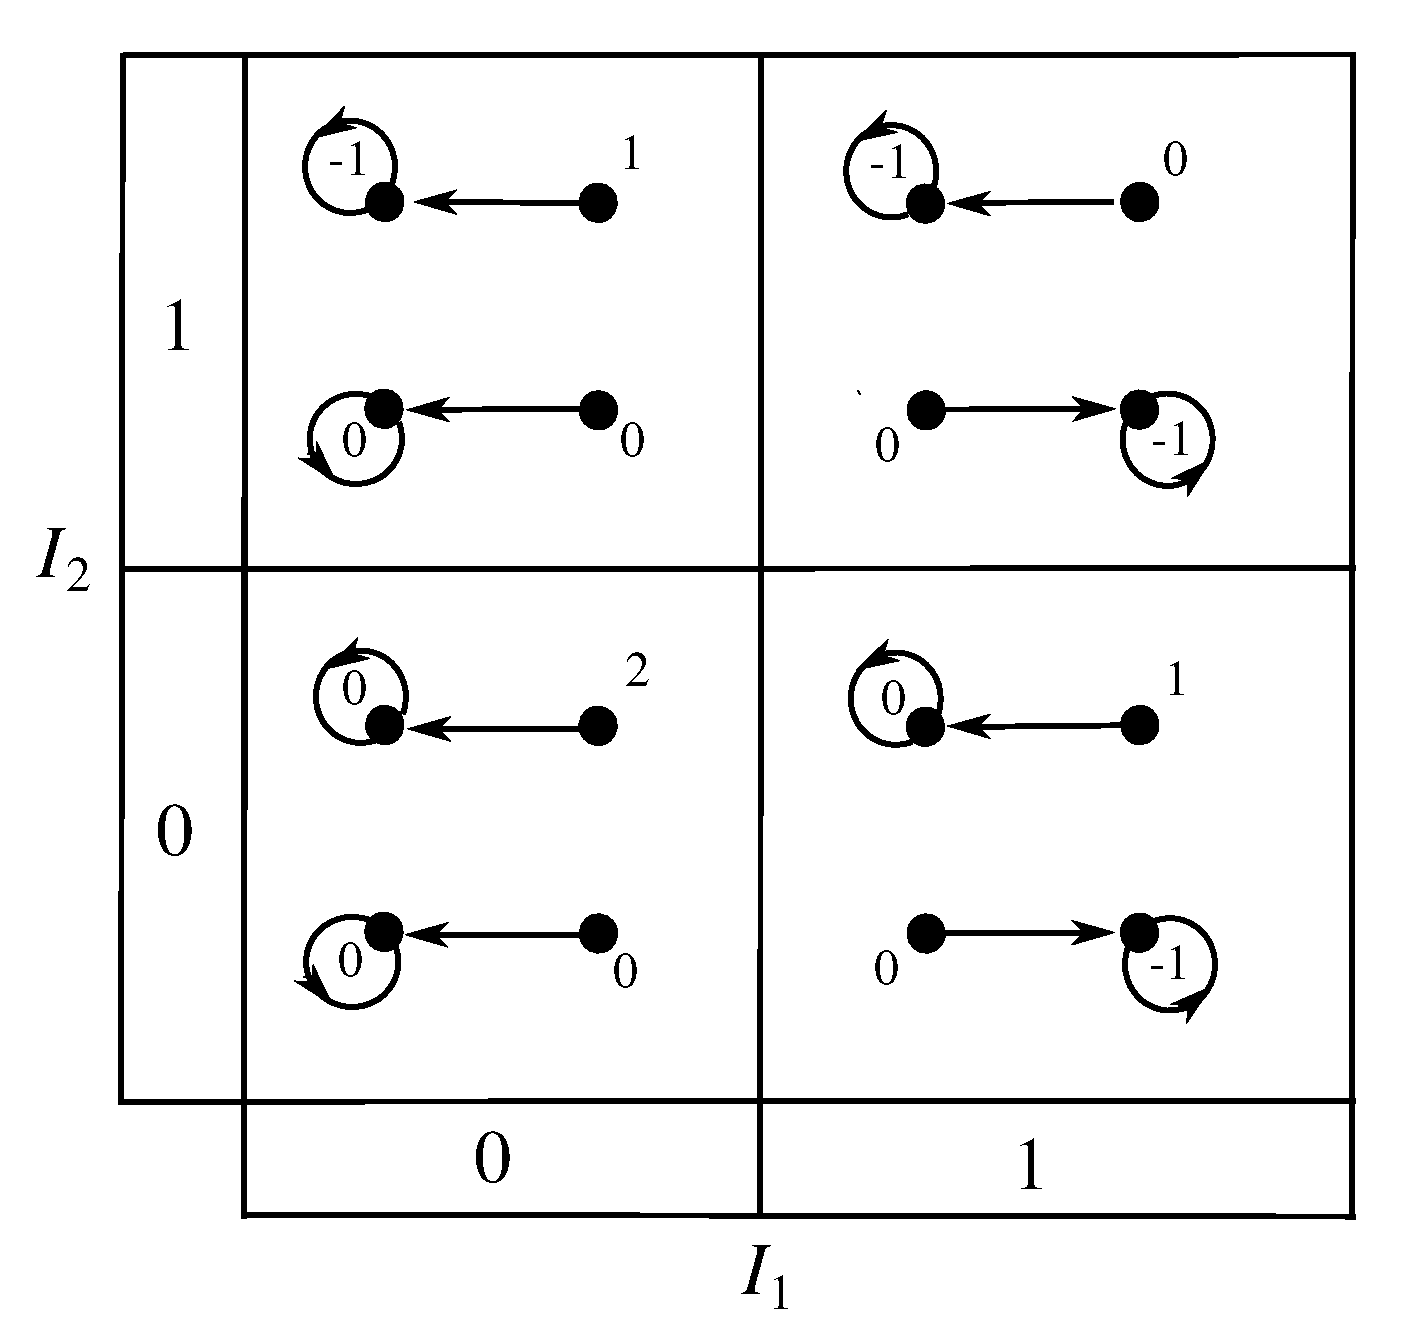
\includegraphics[scale=0.342]{./images/TwoNodeHopfieldUpdate1.pdf}
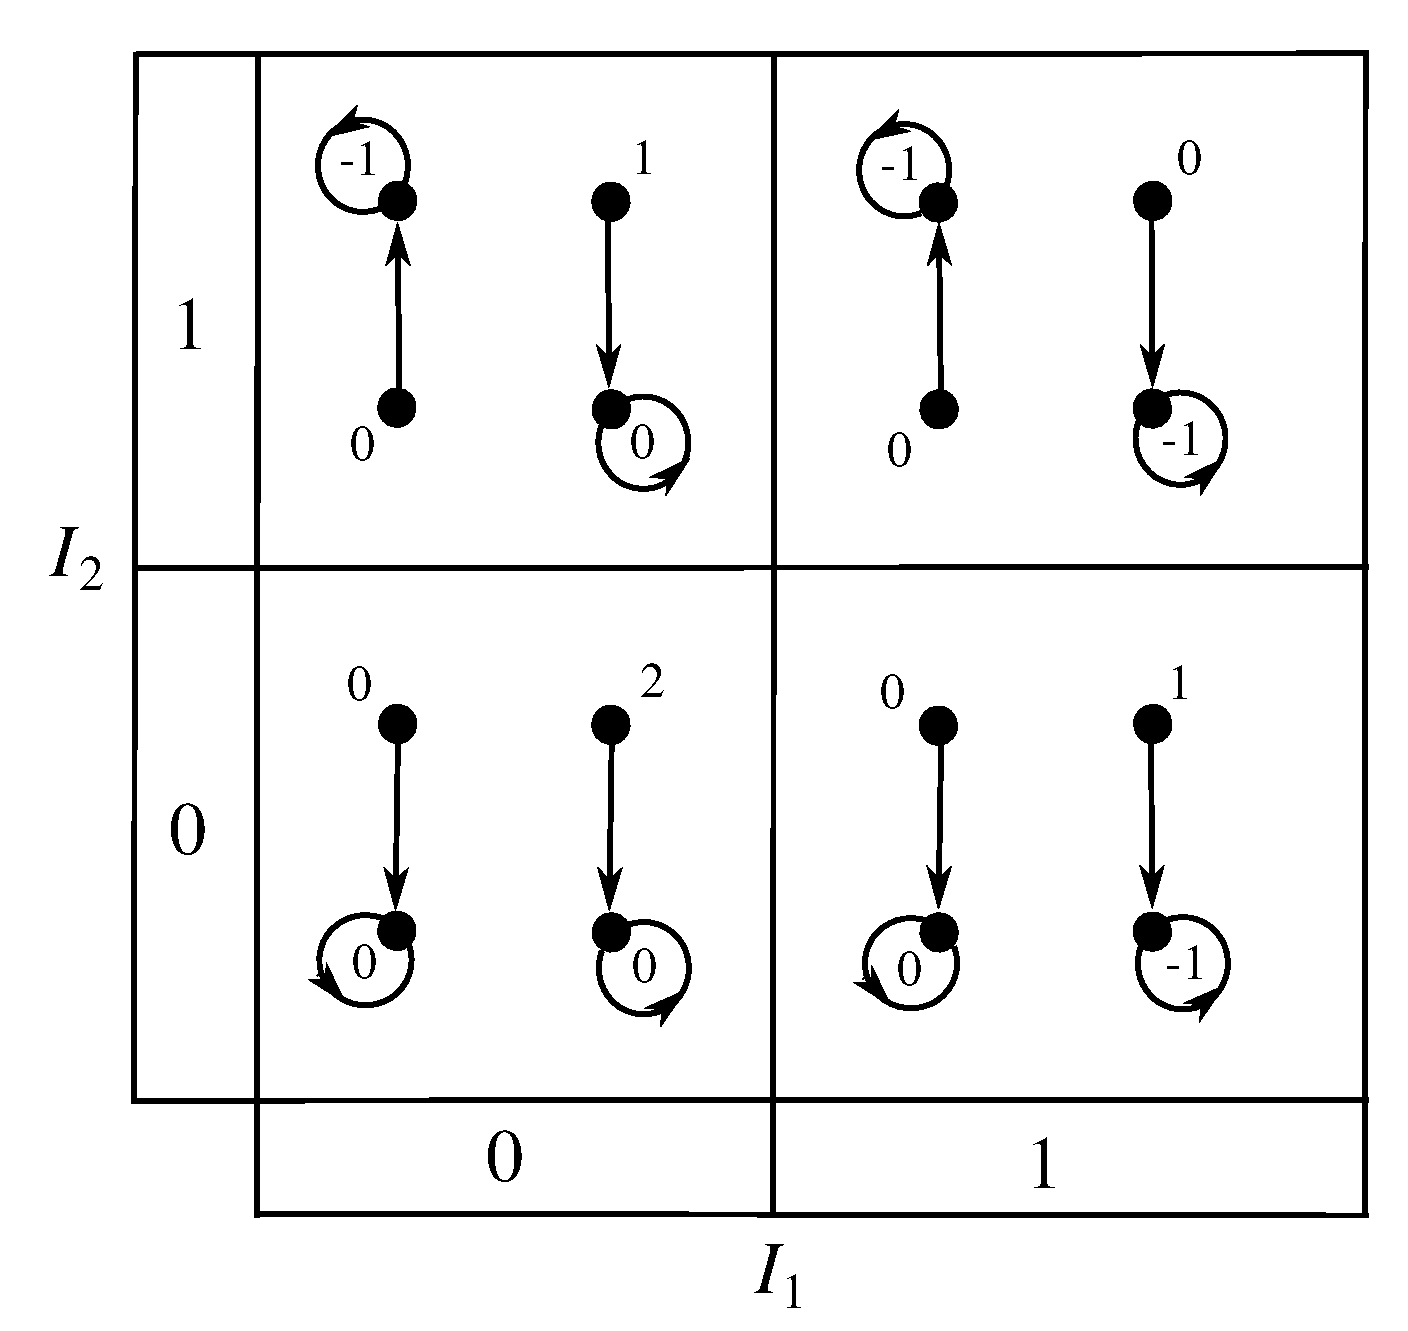
\includegraphics[scale=0.342]{./images/TwoNodeHopfieldUpdate2.pdf}
\caption{Digraphs for the functions on the state space $\{0,1\}^2$ when only 
one neuron is updated at time.  The value of the potential function 
$V(y_1,y_2)$ is labeled next to each state.  (Left) The digraphs for the 
function $F_1$, only neuron 1 can change its activation.  (Right) The digraphs 
for the function $F_2$, only neuron 2 can change its activation.  For each 
input vector there are two attracting fixed points.  Which fixed point the 
system ends up in depends on the initial state.  If the input vector is not 
$(1,1)^T$ the fixed point may or may not match the input.  If the input vector 
is $(1,1)^T$ then the fixed points do not match the input.}
\label{F:TwoNodeHopfieldSingle}
\end{figure}

  In addition Fig. \ref{F:TwoNodeHopfieldSingle} shows that $F_1$ and $F_2$ 
never increase the value of the potential function $V(y_1,y_2)$.  So composing 
them never increases the value of $V(y_1,y_2)$.  In this respect asynchronous
update is like synchronous update.

\subsubsection{Sequential update} 

  With just two nodes there are just two possible sequences for the nodes.
We either start with neuron $1$ and go to neuron $2$ or we start with neuron 
$2$ and go to neuron $1$.  
\begin{eqnarray*}
\begin{pmatrix}
y_1(t+1) \\ y_2(t+1)
\end{pmatrix}
= 
F_{12}
\left(
\begin{pmatrix}
y_1(t) \\ y_2(t)
\end{pmatrix},
\begin{pmatrix}
I_1 \\ I_2
\end{pmatrix}
\right)
=
F_1
\left(
F_2
\left(
\begin{pmatrix}
y_1(t) \\ y_2(t)
\end{pmatrix},
\begin{pmatrix}
I_1 \\ I_2
\end{pmatrix}
\right),
\begin{pmatrix}
I_1 \\ I_2
\end{pmatrix}
 \right) \\
\begin{pmatrix}
y_1(t+1) \\ y_2(t+1)
\end{pmatrix}
= 
F_{21}
\left(
\begin{pmatrix}
y_1(t) \\ y_2(t)
\end{pmatrix},
\begin{pmatrix}
I_1 \\ I_2
\end{pmatrix}
\right)
=
F_2
\left(
F_1
\left(
\begin{pmatrix}
y_1(t) \\ y_2(t)
\end{pmatrix},
\begin{pmatrix}
I_1 \\ I_2
\end{pmatrix}
\right),
\begin{pmatrix}
I_1 \\ I_2
\end{pmatrix}
 \right)
\end{eqnarray*}
The digraphs for these two functions are shown in Fig.  
\ref{F:TwoNodeHopfieldSequence}.  We can obtain the digraph for $F_{12}$ by
seeing where states go in the digraph for $F_2$ in Fig. 
\ref{F:TwoNodeHopfieldSingle} and then where those states go in the digraph for
$F_1$.  To obtain the digraph for $F_{21}$ we look at where states go in the
digraph for $F_1$ and then where those states go in the digraph for $F_2$.

\begin{figure}[ht]
\centering
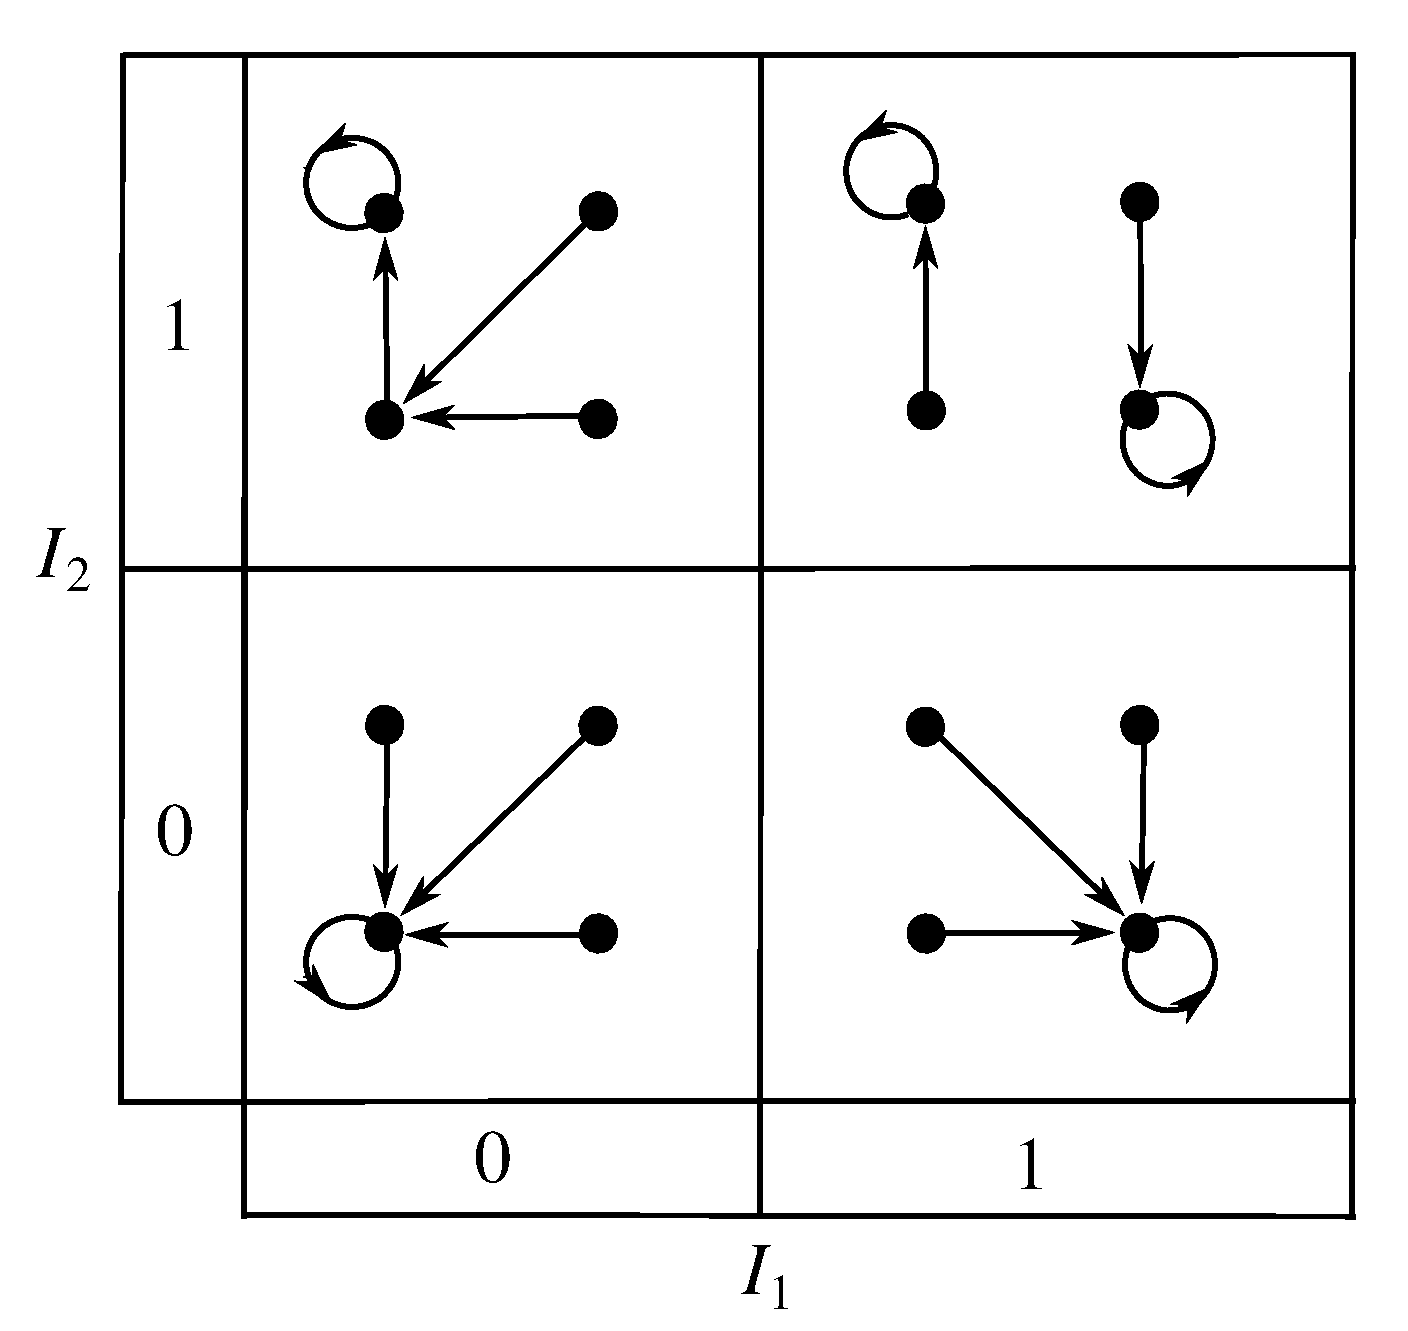
\includegraphics[scale=0.342]{./images/TwoNodeHopfieldUpdate12.pdf}
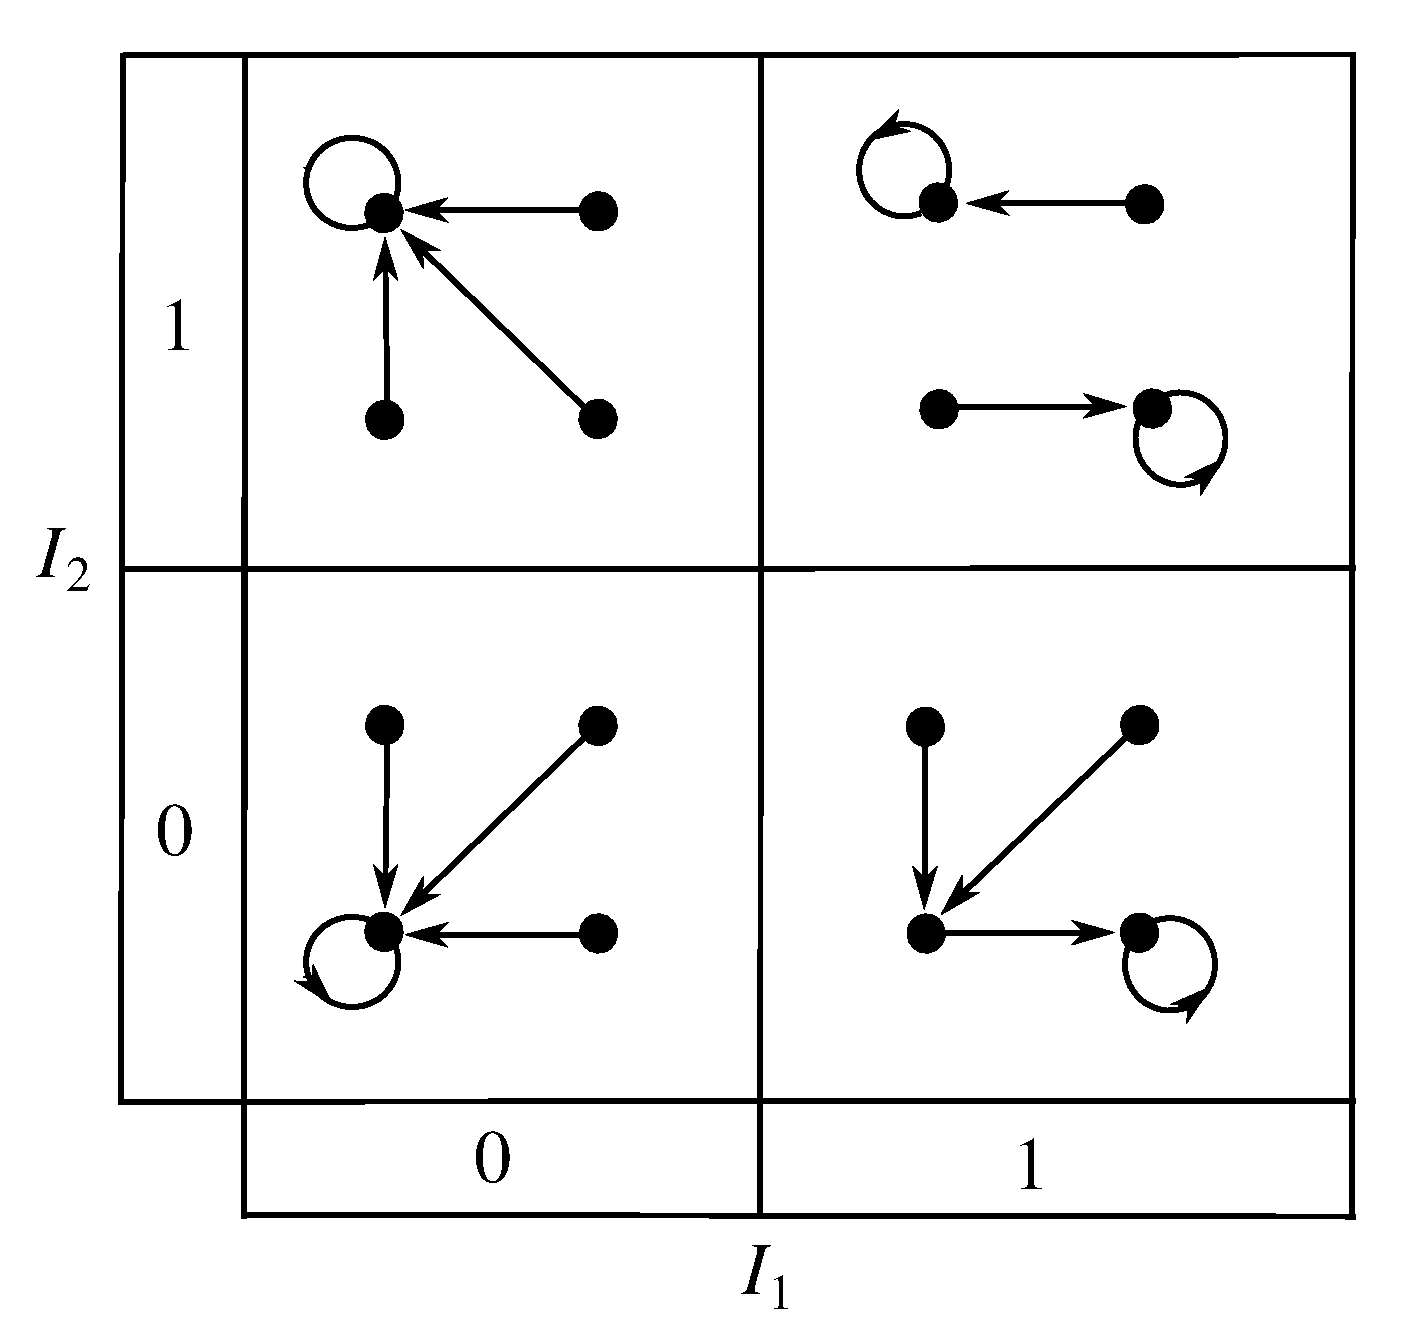
\includegraphics[scale=0.342]{./images/TwoNodeHopfieldUpdate21.pdf}
\caption{Digraphs for the dynamical systems obtained by sequential update. 
(Left) The dynamical systems obtained by iterating $F_{12}$ for each input.  
(Right) The dynamical systems obtained by iterating $F_{21}$ for each input.  
If the input vector is not $(1,1)^T$ then the system has a globally attracting 
fixed point and it matches the input vector.  If the input vector is $(1,1)^T$ 
then the fixed points are $(1,0)$ and $(0,1)$.  Which fixed point the system 
ends up in depends on the initial state.}
\label{F:TwoNodeHopfieldSequence}  
\end{figure}

   As with synchronous update the dynamical systems obtained by iterating 
$F_{12}$ or $F_{21}$ go to the fixed point we want for the input so long as 
the input vector is not $(1,1)^T$.  If the input vector is $(1,1)^T$ then the 
dynamical systems go to one of the fixed points $(1,0)^T$ or $(0,1)^T$.  Unlike
with synchronous update neither $F_{12}$ nor $F_{21}$ produce oscillations in 
the state space.  If both inputs are $1$ the network will recognize the 
presence of just one of the objects.  Which object it detects depends on the 
initial state and the order in which we update the neurons.

\subsubsection{Stochastic update} 

   In stochastic update we select which neuron to update randomly.  In this 
section we will use a uniform probability function to make the selection.  
So the probability for each neuron being selected is $1/2$.  The functions 
$F_1$ and $F_2$ are the update functions for neuron 1 and neuron 2 
respectively.  To analyze stochastic update it is useful to combine the 
digraphs for $F_1$ and $F_2$ in Fig. \ref{F:TwoNodeHopfieldSingle} into a
single digraph.  This union of digraphs is shown in Fig. 
\ref{F:TwoNodeHopfieldStochastic}.  
   
   The functions $F_1$ and $F_2$ have the same domain and range which is the
set of vertices of a square.  So each of the digraphs for $F_1$ and $F_2$ have 
the same set of vertices which is $\{0,1\}^2$.  The digraphs for $F_1$ and 
$F_2$ only differ in having some of their directed edges be different.   

   Because the digraphs stand for functions each vertex has exactly one edge 
directed away from it.  If $F_1$ and $F_2$ have the same value at a vertex then
their digraphs have the same edge directed away from that vertex.  In the 
union of the digraphs for $F_1$ and $F_2$ this vertex has just that one edge
directed away from it.  If $F_1$ and $F_2$ do not have the same value at a 
vertex then their digraphs have different edges directed away from that vertex.
In the union of the digraphs for $F_1$ and $F_2$ this vertex has these two 
edges directed away from it.  This can be checked in Figs. 
\ref{F:TwoNodeHopfieldSingle} and \ref{F:TwoNodeHopfieldStochastic}.  

\begin{figure}[ht]
\centering
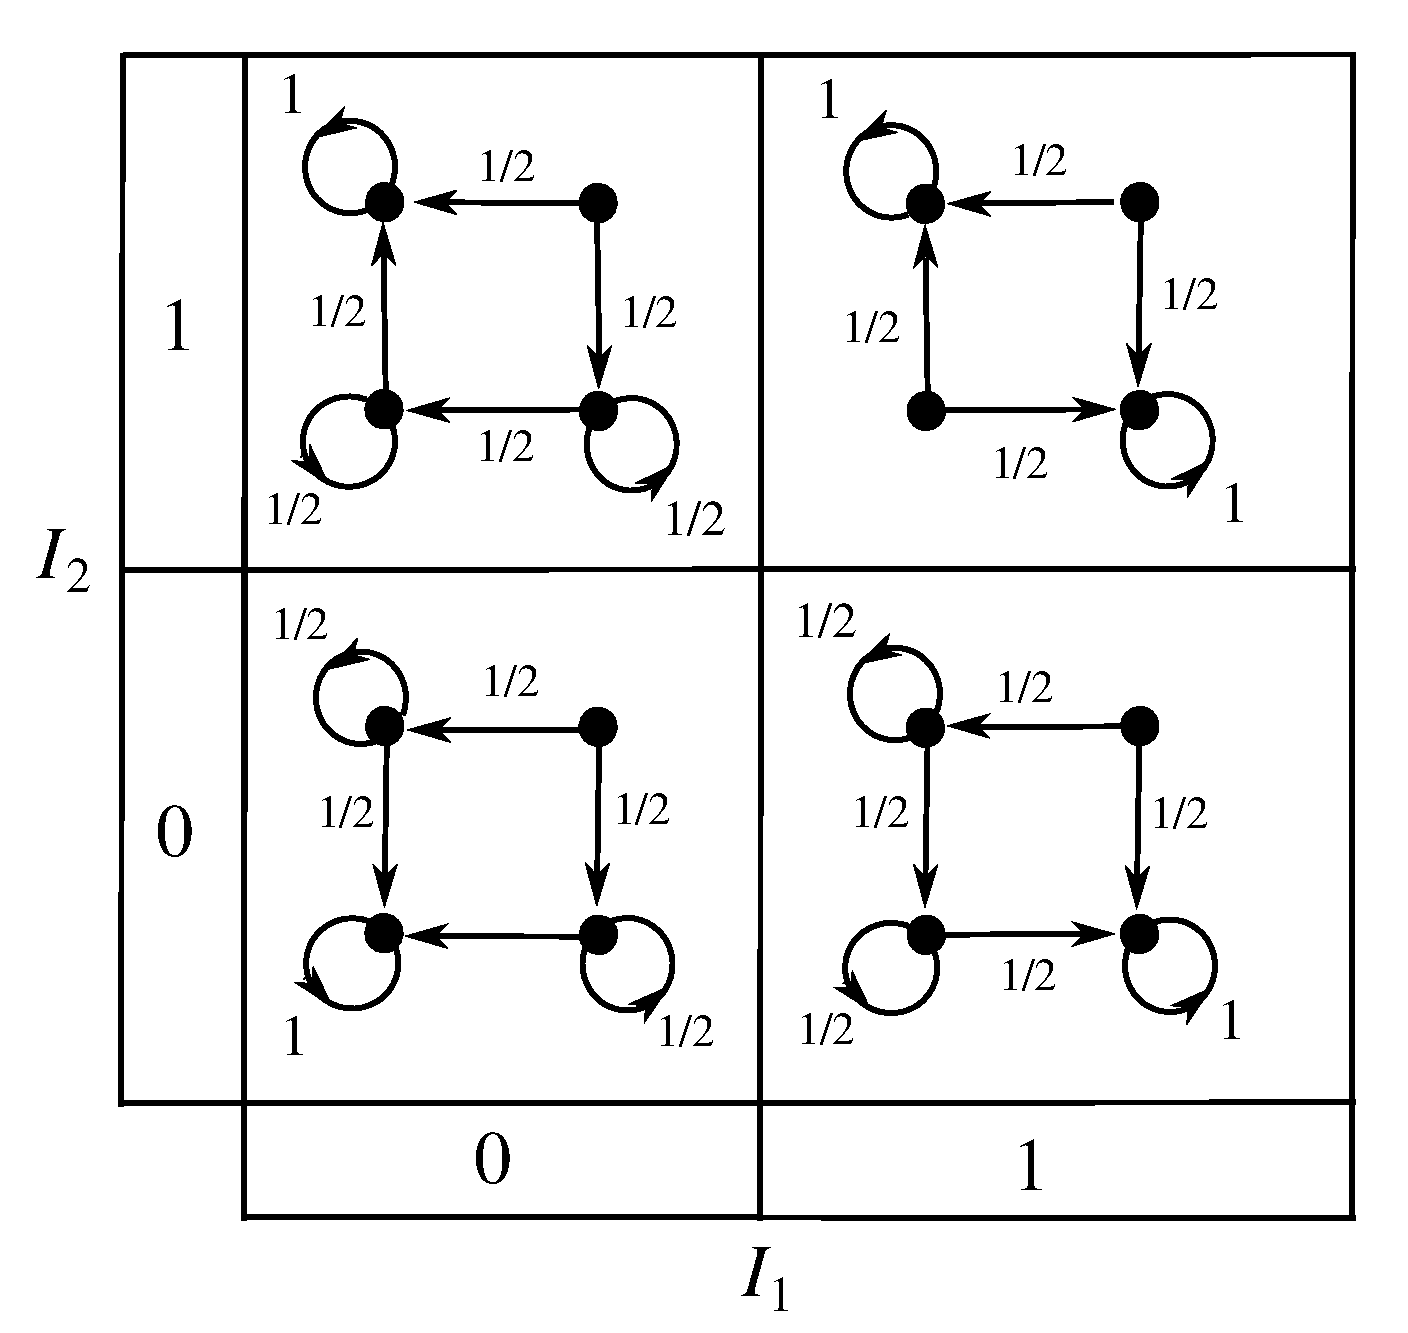
\includegraphics[scale=0.45]{./images/TwoNodeHopfieldMarkov.pdf}
\caption{Stochastic update where the neuron to update is randomly selected with 
a probability of $1/2$ is represented with a transition diagram.  The states
are indicated by the dots and the arrows between the dots indicate the possible 
transitions between states.  Each arrow is labeled with the probability that the
transition will occur.  If the input vector is not $(1,1)^T$ then the system 
eventually reaches the state that matches its input.  If the input vector is 
$(1,1)^T$ and the system starts out in $(1,0)^T$ or $(1,0)^T$ then it will
stay in its starting state, otherwise it eventually reaches either $(1,0)^T$ or 
$(1,0)^T$ with probability of $1/2$, and stays there.} 
\label{F:TwoNodeHopfieldStochastic}  
\end{figure}

   When $F_1$ and $F_2$ have the same value at a vertex then the probability 
that the network will transition to that state is $1$.  In the union of the
digraphs for $F_1$ and $F_2$ we label the edge directed away from the vertex
with a $1$ to indicate that the probability for that transition to occur is 
$1$.  

   When $F_1$ and $F_2$ have different values at a vertex then there are two 
states the network can transition to.  Since the probability for a neuron to be
selected is $1/2$ the probability for each of the transitions is $1/2$.  In the 
union of the digraphs for $F_1$ and $F_2$ we label the two edges directed away 
from the vertex with $1/2$ to indicate that the probability for that transition 
to occur is $1/2$.

   These digraphs with their edges labeled with probabilities are known as 
transition digraphs, transition graphs, and as transition diagrams for a Markov
process.  As we said at the beginning of this section a Markov process is a 
stochastic process for which future states only depend on the present state.  A 
Hopfield network with stochastic update is a Markov process.  The future states 
of a Hopfield network only depend on the present state and how the neurons are 
randomly selected to be updated.  Fig. \ref{F:TwoNodeHopfieldStochastic} shows 
the transition diagram for the Markov process in this example Hopfield network.

   There is a well developed theory for Markov processes but the Markov
processes in this example Hopfield network are particularly simple cases of 
Markov processes.  So we will not need to use very much from the theory of 
Markov processes.

   If the only edge directed from a vertex is also directed towards itself then
the vertex is called an absorbing state of the Markov process.  The presence of
absorbing states simplifies the analysis of a Markov process.  Once a Markov 
process reaches an absorbing state it does not leave.  

   It can be seen from the transition diagram that when the input vector is not 
$(1,1)^T$ there is exactly one absorbing state in the neural network's state 
space.  Moreover each of these absorbing states matches the input vector.  When 
the input vector is $(1,1)^T$ there are two absorbing states, $(1,0)^T$ and 
$(0,1)^T$.

   It can be seen from the transition diagram that the neural network state 
$(1,1)^T$ has no edges directed towards it.  This means that the neural 
network can not remain in the state $(1,1)^T$ and once it leaves it does not 
return.

  It can also be seen from the transition diagram that, except for the state
$(1,1)^T$, each of the non-absorbing states can transition to themselves.  For 
each of these non-absorbing states there are no other directed paths in the 
digraph that begin and end with them.  Once the Hopfield network leaves one of these states it does not return.

   For each of the non-absorbing states that can transition to themselves the
probability that it will transition to itself in one time step is $1/2$.  The
probability that it will transition to itself in two time steps is $(1/2) \cdot
(1/2) = 1/4$.  The probability that it will transition to itself in $k$ time 
steps is $1/2^k$.  This probability goes to $0$ as $k$ is increased without
bound.  So as we keep performing stochastic update the probability that it
will transition away from itself goes to $1$.  We say it is almost certain that
it will transition away from itself.  This is like flipping a coin until it
stops landing heads.  It is almost certain that sooner or later you will stop 
flipping the coin.

   So eventually the Hopfield networks will transition away from each 
non-absorbing state without returning.  Therefore they eventually end up in an 
absorbing state.  When the input vector is not $(1,1)^T$ there is a unique 
absorbing state and it matches the input vector.  When the input vector is 
$(1,1)^T$ the absorbing states are $(1,0)^T$ and $(0,1)^T$.  If the neural 
network does not begin in one of these absorbing states then which one it ends 
up in is random.  The probability of ending up in one of these two absorbing 
states is $1/2$.

  With stochastic update the Hopfield network can recognize the absence of
both objects and it can recognize the presence of one object when the other
object is not present.  If both objects are present it random enters one of the
states for the presence of a single object.

\subsubsection{Summary}

   In summary the long term behavior for the synchronous, sequential, and 
stochastic update methods is the same when the input vector is not $(1,1)^T$.  
The system goes to the state that matches the input and stays there.  When the 
input vector is $(1,1)^T$ the points $(0,0)^T$ and $(1,1)^T$ form a 2-cycle of 
the dynamical system for synchronous update but for sequential and stochastic 
update the network eventually ends up in either the state $(1,0)^T$ or the 
state $(0,1)^T$.